There are multiple solutions to the Einstein field equations. Details of their derivations are left to the reader, but a quick summary of a few important ones are given here.
\section{Schwarzschild Solution}
One of the first big solutions was the Schwarzschild solution, published in 1916 by Karl Schwarzschild. The solution showed the existence of an object
now called a black hole. A black hole is an object so massive that not even light can escape from it. Black holes are a subject of intense research today,
and it is believed that many stars collapse to become black holes after they die. This was in fact predicted by Chandrasekhar, with his idea of mass
determining what stars became when they died. Black holes have also seen further research in terms of gravitational waves (see section 5.3). 
The other interesting thing about black holes is that while general relativity predicted their existence, general relativity cannot explain the inside
of black holes. This is a large problem for future researchers (it ties in with the problems between general relativity and the other major
scientific theory of the 20th century, quantum mechanics). 
\section{Big Bang}
One of the more famous solutions to general relativity, the Big Bang was originally called the cosmic egg by Georges Lemaitre, who published 
his solution to the equations in 1927. While Einstein originally pronounced Lemaitre's theory nonsense (the accepted theory of the day 
was that the universe had lasted and was going to last for forever), it was eventually accepted. Edwin Hubble's evidence, found in 1929,
of redshift among galaxies showed that they were indeed moving apart and the universe was expanding. The detection of cosmic background radiation (CMB) 
was another important piece of evidence in favor of the Big Bang's occurrence. Today, the Big Bang, as well as much of the 
rest of general relativity forms the foundation for the field of cosmology. The Big Bang is the idea that the universe originally started
as a point, with infinite mass, and then expanded very rapidly, eventually allowing atoms, stars, galaxies, planets, and so forth to form.
A general diagram showing the time frame of the Big Bang is given below.
\begin{figure}[H]
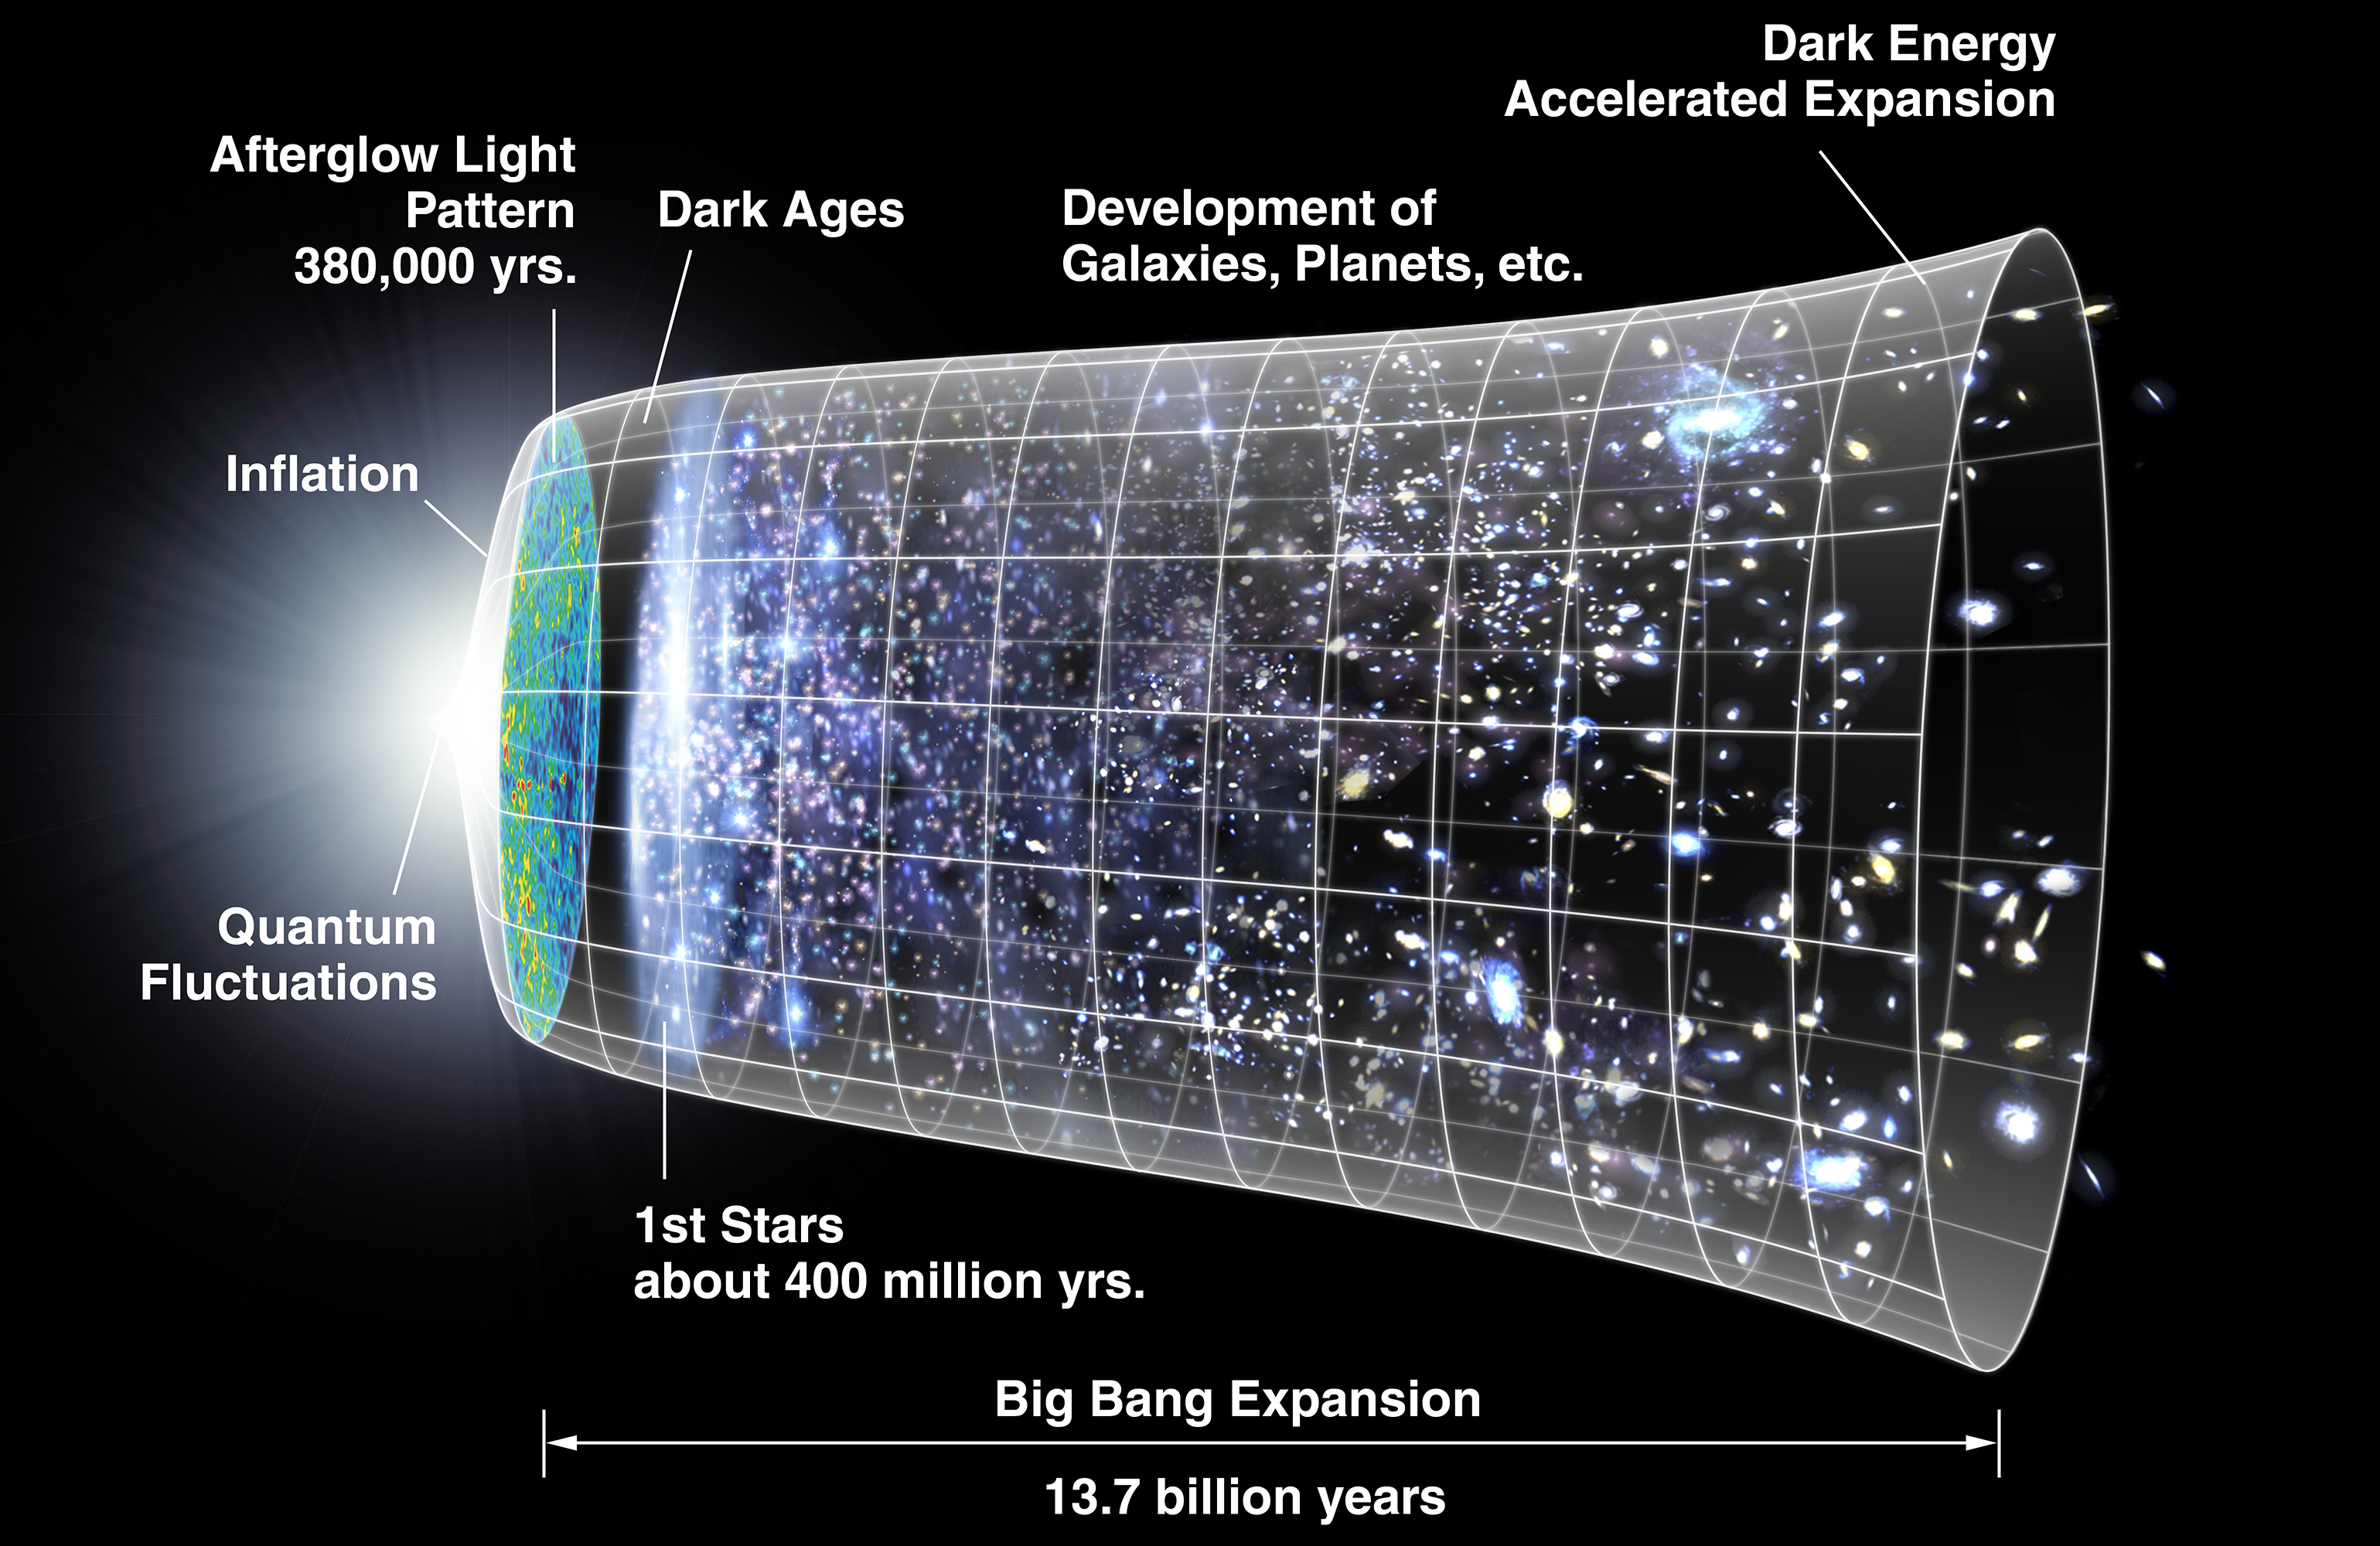
\includegraphics[scale=0.1]{bigbang.jpg}
\end{figure}
The Big Bang theory is subject to much controversy, and no one can explain how the Big Bang started. 
\section{Gravitational Waves}
Just this past year (as of January 2017) LIGO announced an extraordinairy breakthrough: detecting gravitational waves. Basically, imagine
two huge black holes colliding and eventually merging. As the black holes come closer and closer, they send out ripples in the fabric
of spacetime, just like waves spread out from an object dropping into a pond. 
\begin{figure}[H]
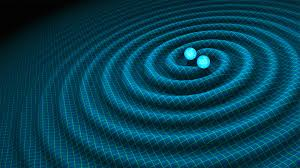
\includegraphics[scale=0.5]{gwaves.jpg}
\end{figure}
These ripples are incredibly strong near the location of the
collision, and warp space and time dramatically. But after they've travelled a long distance, they are incredibly weak, changing distances
no more than the width of an atom's nucleus. So detecting these waves is incredibly hard. The way LIGO does it is by sending a laser beam
through a beam splitter, and then the laser beams travel down two very long arms that are precisely the same length. At the end, the beams bounce back and head back toward the beginning of the 
L shape. If they arrive back at precisely the same time, they pass through a special piece of equipment that makes the laser beams cancel out.
If they arrive at slightly different times, though, both beams keep going and hit a detector that senses whether light has hit it.
If light has, one of the arms has shortened or lengthened by a tiny amount due to the gravitational wave, therefore showing that a gravitational
wave has passed through.
\begin{figure}[H]
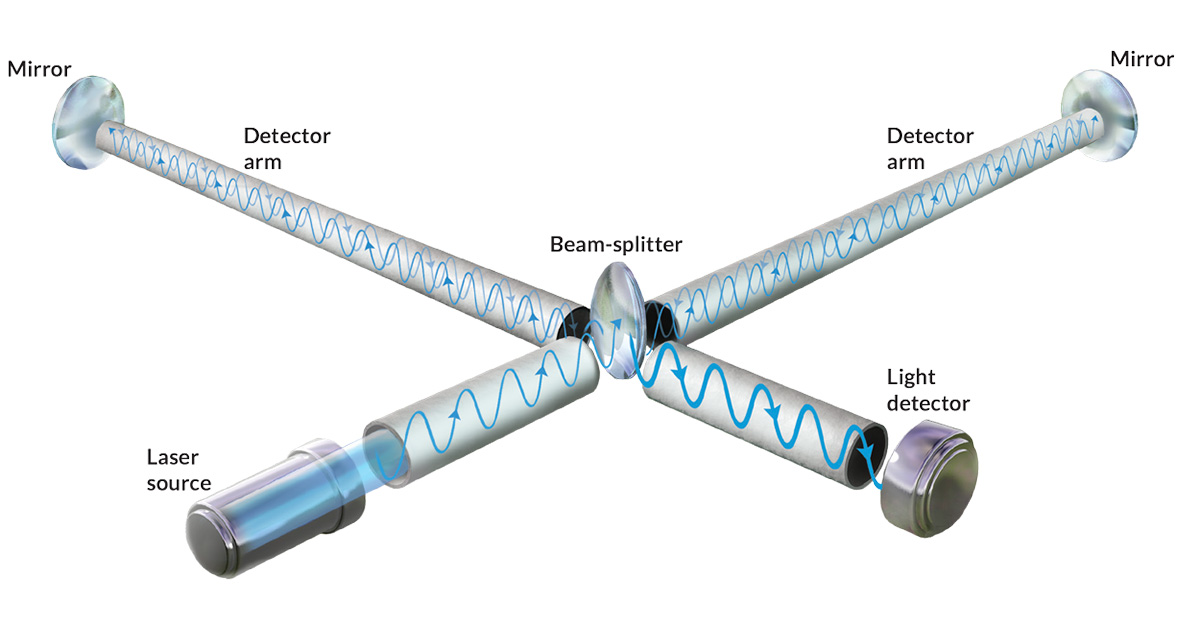
\includegraphics[scale=0.25]{ligo.jpg}
\end{figure}
There are two of these instruments on opposite sides of the United States, therefore preventing something like an earthquake from messing with
the results (if the two instruments both detect a gravitational wave, it is highly unlikely something affected both at the same time).
A solution of the field equations has also been found that predicts gravitational waves.
